\chapter{Spezielle Relativitätstheorie: Bezugssysteme, Gleichzeitigkeit und die Lorentz-Transformation}

Relativität ist das Prinzip, dass die Gesetze der Physik nicht davon abhängen, welches Inertialsystem wir zu ihrer Beschreibung verwenden. Unsere erste Aufgabe ist die Kinematik: die Bedeutung von Raum, Zeit, Bewegung, Synchronisation und der Transformation von einem Inertialsystem in ein anderes. Danach folgt die Dynamik mit relativistischer Energie, relativistischem Impuls, Kraft, dem Analogon zu Newtons Bewegungsgleichung und der Bedeutung von \(E=mc^2\). Sobald dieses Gerüst gesichert ist, können wir uns der allgemeinen Relativitätstheorie konzeptionell über die gekrümmte Raumzeit, die Bewegung von Teilchen in einem vorgegebenen Gravitationsfeld, Schwarze Löcher und die Expansion des Universums nähern, ohne mit dem schwierigen Problem zu beginnen, Einsteins Feldgleichungen zu lösen.

Es lohnt sich, zwischen konzeptioneller und mathematischer Strenge zu unterscheiden. Wir werden keine Näherung verwenden, von der wir wissen, dass sie falsch ist. Stattdessen betonen wir, wie ein Gravitationsfeld auf Uhren, Teilchen und Geometrie wirkt, und verschieben die mathematischen Werkzeuge, die nötig sind, um beliebige Lösungen der Feldgleichungen zu konstruieren. Die spezielle Relativitätstheorie muss ausführlicher behandelt werden, weil alle späteren Überlegungen auf ihrer Kinematik beruhen.

Der richtige Ausgangspunkt ist daher nicht eine berühmte Formel, sondern eine präzise Darstellung dessen, was ein Beobachter unter einem Ort und einer Zeit versteht.

\section{Ein Bezugssystem ist ein physikalisches Koordinatensystem}

Stellen wir uns vor, der Raum sei mit einem beliebig feinmaschigen Gitter aus Meterstäben ausgefüllt. Jeder Gitterpunkt ist durch drei räumliche Koordinaten gekennzeichnet, und an jedem Punkt befindet sich eine Uhr. Zusammen bilden Stäbe und Uhren ein Bezugssystem.

\begin{definition}Ein \emph{Ereignis} ist etwas, das an einem Ort und zu einer Zeit geschieht. In einer räumlichen Dimension schreibt man seine Koordinaten als \((x,t)\), in drei Dimensionen als \((x,y,z,t)\).
\end{definition}

Die Newtonsche Physik fügt eine weitreichende Annahme hinzu: Alle idealen Uhren lassen sich ein für alle Mal synchronisieren. Die Zeit ist universell. Eine Uhr kann bewegt werden, und ein Beobachter kann eine Taschenuhr bei sich tragen, doch alle sollen überall dieselbe \(t\) angeben. Dies nennt man mitunter absolute Zeit; man kann sie sich als Gotteszeit vorstellen, als eine einzige Uhr für die ganze Welt.

Das Relativitätsprinzip ist älter als Einstein. Ein anschauliches Bild dafür ist ein Zug, der sich so gleichmäßig auf vollkommen glatten Schienen bewegt, dass nichts rattert oder wackelt. Im Zug können wir Bälle genauso zuwerfen und auffangen wie in einem Zug, der am Bahnhof steht. Jonglieren ist ein erstaunlich vollständiges kleines Mechanikexperiment: Es erfordert Zeitmessung, Schwerkraft, Ausrichtung und wiederholte Kontrolle von Flugbahnen. Bewegt sich der Zug mit konstanter Geschwindigkeit, ändert sich keine dieser Regeln. Ein senkrecht nach oben geworfener Ball kehrt in dieselbe Hand zurück; der Zug gleitet nicht unter ihm weg. Galileo erkannte diesen Sachverhalt, und Newton brachte ihn systematisch in seinen Bewegungsgesetzen zum Ausdruck.

Vor Galileo lag der Gedanke nahe, der fahrende Zug müsse während des Fluges des Balls weiterfahren, sodass der Jongleur die Hand nach hinten oder vorn bewegen müsse, um ihn wieder aufzufangen. Der Fehler dabei ist, zu vergessen, dass der Ball beim Verlassen der Hand bereits die horizontale Geschwindigkeit des Zuges besitzt. Kein Experiment, das auf den gleichmäßig fahrenden Wagen beschränkt ist, kann einen besonderen Zustand absoluter Ruhe nachweisen. Beobachtbar ist nur die Relativbewegung zwischen den beiden Zügen.

Der stehende und der sich gleichförmig bewegende Zug sind daher zwei Inertialsysteme. Vor Einstein waren sie durch Galilei-Transformationen miteinander verknüpft.

\section{Raumzeit zeichnen}

Zunächst lassen wir \(y\) und \(z\) weg und tragen die Zeit vertikal und den Ort \(x\) horizontal auf. Jeder Punkt in der Zeichnung ist ein Ereignis. Die Linie \(x=0\) ist die Geschichte oder die \emph{Weltlinie} des räumlichen Ursprungs. Die benachbarten vertikalen Linien \(x=1,2,3,\ldots\) sind die Weltlinien der übrigen Gitterpunkte. Horizontale Linien umfassen Ereignisse mit gleicher Zeit.

\begin{figure}[H]
\centering
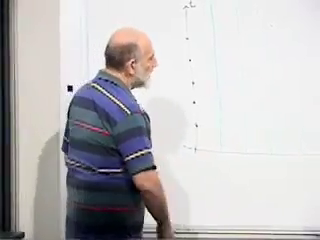
\includegraphics[width=0.62\textwidth]{lecture_01_figure_02.png}
\caption{Die Zeitachse des Ruhesystems und die ersten Weltlinien des räumlichen Gitters.}
\lectureframe{00:16:38}
\end{figure}

Dieselbe Konstruktion lässt sich in einer idealisierten Zeichnung anschaulicher darstellen:

\begin{figure}[H]
\centering
\begin{tikzpicture}[scale=0.95]
\draw[->] (-1.2,0) -- (5.2,0) node[right] {$x$};
\draw[->] (0,-0.2) -- (0,4.8) node[above] {$t$};
\foreach \x in {-1,1,2,3,4}
  \draw[gray!65] (\x,0) -- (\x,4.4);
\foreach \y in {1,2,3,4}
  \draw[gray!65] (-1.0,\y) -- (4.4,\y);
\fill (0,0) circle (1.5pt);
\node[below left] at (0,0) {$0$};
\node[left] at (0,1) {$1$};
\node[left] at (0,2) {$2$};
\node[left] at (0,3) {$3$};
\node[below] at (1,0) {$1$};
\node[below] at (2,0) {$2$};
\node[below] at (3,0) {$3$};
\end{tikzpicture}
\caption{Ein ruhendes Raumzeitgitter. Vertikale Linien haben konstanten Ort, horizontale Linien konstante Zeit.}
\end{figure}

Das Gitter ist imaginär, und sein Abstand ist beliebig. Wir können Meter, Zentimeter, Mikrometer oder ein noch kleineres Intervall verwenden, sofern es physikalisch sinnvoll ist. Es dient dazu, jedem Ereignis eine präzise Koordinate zuzuordnen.

Der Begriff „Bezugssystem“ hat nun eine operationale Bedeutung. Er bezeichnet nicht bloß einen Standpunkt oder eine Person, die in eine bestimmte Richtung blickt, sondern einen ausgedehnten Koordinatenapparat. Zu einem Ereignis geben die örtlichen Stäbe an, wo es stattgefunden hat, und die örtliche Uhr, wann. Dann lassen sich auch andere physikalische Größen zwischen Bezugssystemen vergleichen: der Ort und die Geschwindigkeit eines Teilchens, seine Energie, vielleicht die Temperatur eines Körpers und schließlich sein Impuls und die Kraft. Am einfachsten ist der Vergleich für \(x\) und \(t\); damit beginnen wir.

Nun bringen wir ein zweites Gitter auf einem Zug an, der sich in positiver \(x\)-Richtung mit konstanter Geschwindigkeit \(v\) bewegt. Wir wählen die Ursprünge so, dass sie bei \(t=0\) zusammenfallen. Der bewegte Ursprung folgt dann
\begin{equation}
x=vt.
\end{equation}
Jeder andere im Zug feste Punkt folgt einer parallelen, geneigten Weltlinie. Ihre Neigung bringt geometrisch lediglich zum Ausdruck, dass sich der Zug mit fortschreitender Zeit weiterbewegt.

Nehmen wir an, der hintere Punkt des Zuges sei der gestrichene Ursprung. Bei \(t=0\) fällt er mit dem Ursprung am Bahnhof zusammen. Zu einem späteren Zeitpunkt \(t\) hat er im Bahnhofssystem die Koordinate \(vt\). Ein benachbartes Ereignis mit der Koordinate \(x\) liegt daher nur \(x-vt\) vom Zugursprung entfernt. Deshalb ergibt sich die Transformation als Subtraktion und nicht als beliebige algebraische Regel.

Seien \((x,t)\) die Koordinaten eines Ereignisses im Bahnhofssystem und \((x',t')\) seine Koordinaten im Zugsystem. Galileo und Newton halten an der universellen Zeit fest:
\begin{equation}
t'=t.
\end{equation}
Während der Zeit \(t\) rückt der bewegte Ursprung um \(vt\) vor. Der Abstand zwischen diesem Ursprung und dem Ereignis beträgt daher
\begin{equation}
x'=x-vt.
\end{equation}
Zusammen ergibt sich
\begin{align}
t'&=t, & x'&=x-vt.
\label{eq:galilean-forward}
\end{align}
Löst man nach den ungestrichenen Koordinaten auf, erhält man die inverse Transformation:
\begin{align}
t&=t', & x&=x'+vt'.
\label{eq:galilean-inverse}
\end{align}

\begin{figure}[H]
\centering
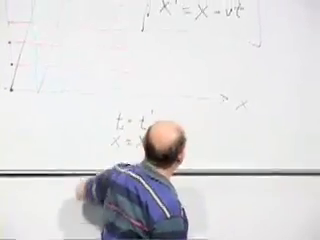
\includegraphics[width=0.72\textwidth]{lecture_01_figure_03.png}
\caption{Die Galilei-Transformation neben den beiden Raumzeitgittern.}
\lectureframe{00:21:57}
\end{figure}

Das erste Gleichungspaar gibt dem bewegten Beobachter an, wie er die Koordinaten des ruhenden Beobachters umrechnet. Das inverse Paar rechnet zurück. Diese wechselseitige Umrechnung der Beschreibungen ist der mathematische Gehalt der Galileischen Relativität.

Die Ersetzung \(t\to t'\) in der inversen Ortsformel ist nur deshalb unproblematisch, weil die Galileische Theorie bereits \(t=t'\) festgelegt hat. Es lohnt sich, diese Annahme jetzt zu beachten. In Einsteins Theorie werden die beiden Zeitkoordinaten verschieden sein, und solche Ersetzungen sind dann nicht mehr selbstverständlich.

\begin{classroomqa}
\audiencequestion{Wenn eine Uhr fortgetragen und dann zurückgebracht wird: Woher wissen wir, dass ihre Bewegung sie nicht zunächst vorgehen und dann nachgehen ließ, sodass der Effekt beim Uhrenvergleich verborgen bleibt?
\lecturetimestamp{00:23:09}}
\lecturerresponse{Galileo hätte die universelle Zeit nicht mit der Präzision moderner Methoden nachweisen können; sie war eine physikalische Vermutung. Wir können sie auf viele Arten prüfen: gute Uhren in entgegengesetzte Richtungen tragen, die Reise sowohl in Nord--Süd- als auch in Ost--West-Richtung wiederholen, eine Uhr um die andere herumführen oder Zeitsignale austauschen, ohne die Uhren zusammenzubringen. Bei gewöhnlichen Geschwindigkeiten stimmen all diese Tests mit sehr hoher Genauigkeit überein. Mit hinreichend genauen Uhren oder hinreichend großen Geschwindigkeiten zeigt sich eine kleine Abweichung. Das Versagen der universellen Zeit ist kein Mangel des Experiments, sondern eines der Phänomene, die die spezielle Relativitätstheorie erklären muss.}
\end{classroomqa}

\section{Galilei-Invarianten und Newtons Gesetz}

Eine Invariante ist eine Größe, über die alle betrachteten Inertialbeobachter übereinstimmen. Die Koordinaten selbst müssen nicht invariant sein. Entscheidend ist, ob die aus ihnen formulierten Gesetze ihre Gestalt behalten.

Das Wort wird sowohl als Substantiv als auch als Adjektiv verwendet. Eine Zahl kann eine Invariante sein, und eine Gleichung kann gegenüber einer Transformation invariant sein. Die Unterscheidung zwischen invarianten Größen und invarianten Gesetzen verhindert ein häufiges Missverständnis: Die Relativitätstheorie behauptet nicht, dass alle Beobachter für alles dieselbe Koordinate erhalten. Sie besagt, dass das physikalische Gesetz, das ihre Messungen verknüpft, dieselbe Form hat.

Betrachten wir zwei gleichzeitige Ereignisse an den Orten \(x_1\) und \(x_2\). Gleichung~\eqref{eq:galilean-forward} ergibt
\begin{align}
x_1'&=x_1-vt,\\
x_2'&=x_2-vt.
\end{align}
Ihr Abstand beträgt daher
\begin{equation}
x_2'-x_1'=(x_2-vt)-(x_1-vt)=x_2-x_1.
\end{equation}
In der Galileischen Physik ist der Abstand zwischen Ereignissen, die zur selben Zeit stattfinden, invariant, obwohl die einzelnen Orte es nicht sind.

\begin{classroomqa}
\audiencequestion{Sind die beiden Vorkommen von \(t\) in dieser Subtraktion wirklich dieselbe Zeit?
\lecturetimestamp{00:28:16}}
\lecturerresponse{Ja. Wir haben die beiden Ereignisse bewusst so gewählt, dass sie \((x_1,t)\) und \((x_2,t)\) sind. Sie liegen auf derselben horizontalen Linie konstanter Zeit. Der gemeinsame Term \(vt\) kürzt sich daher heraus. Fänden die Ereignisse zu unterschiedlichen Zeiten statt, wäre mit diesem Argument kein invariantes räumliches Intervall nachgewiesen.}
\end{classroomqa}

Beschreiben wir nun ein Teilchen durch eine Bahn \(x(t)\). Der Beobachter im Zug ordnet ihm zu:
\begin{equation}
x'(t)=x(t)-vt.
\end{equation}
Einmaliges Ableiten ergibt die bekannte Additionsregel für Geschwindigkeiten:
\begin{equation}
\frac{dx'}{dt}=\frac{dx}{dt}-v.
\end{equation}
Ort und Geschwindigkeit hängen vom Bezugssystem ab. Ein Beobachter, der neben einem Pfeil herfährt, sieht ihn langsamer fliegen als ein Beobachter, der neben der Strecke steht.

Leiten wir ein zweites Mal ab. Da die Relativgeschwindigkeit \(v\) konstant ist, gilt
\begin{equation}
\frac{d^2x'}{dt^2}=\frac{d^2x}{dt^2}.
\end{equation}
Die Beschleunigung ist unter einer Galilei-Transformation invariant. Das legt nahe, weshalb Newtons Gesetz mit der Beschleunigung und nicht mit Ort oder Geschwindigkeit formuliert wird.

Gemeint ist die Beschleunigung eines beobachteten Objekts, nicht die Beschleunigung des Zugbeobachters. Beide Bezugssysteme sind Inertialsysteme, also beschleunigt keines relativ zum anderen. Objekte können sich innerhalb beider Beschreibungen nach links oder rechts beschleunigen, und die beiden Beobachter stimmen im Wert dieser Beschleunigung überein, obwohl sie sich über den Ort und die Geschwindigkeit des Objekts uneinig sind.

Nehmen wir an, zwei Teilchen üben Kräfte aufeinander aus, und die Kraft hängt nur von ihrem gleichzeitigen Abstand ab. Dieser Abstand ist invariant, also ist auch die Kraft invariant. Wenn die Masse außerdem eine intrinsische, bezugssystemunabhängige Eigenschaft ist, kann jeder Inertialbeobachter schreiben:
\begin{equation}
F=ma
\end{equation}
und zwar genau in derselben Form. Die Newtonsche Mechanik ist unter Galilei-Transformationen invariant. Das ist nicht bloß plausibel; im Bereich gewöhnlicher Geschwindigkeiten ist sie außerordentlich genau.

Das Argument gilt für vertraute Zentralkräfte wie die Newtonsche Gravitation oder die Elektrostatik, deren Betrag eine Funktion des Abstands ist. Da alle Galilei-Beobachter bei gleicher Zeit in diesem Abstand übereinstimmen, stimmen sie auch in der Kraft überein. Wenn Kraft und Beschleunigung feststehen, müssen sie für Konsistenz auch in der Masse übereinstimmen: Ein Ein-Kilogramm-Objekt bleibt ein Ein-Kilogramm-Objekt, wenn es auf einem Zug an ihnen vorbeigetragen wird. Jedes Symbol in \(F=ma\) fügt sich in dieselbe invariante Struktur ein.

\section{Licht folgt nicht der Galileischen Regel}

Der Elektromagnetismus führt zu einer Schwierigkeit. Maxwells Gleichungen sagen Wellen voraus, die sich im leeren Raum mit einer bestimmten Geschwindigkeit \(c\) ausbreiten. Sind Maxwells Gleichungen Naturgesetze und gelten die Naturgesetze in jedem Inertialsystem in gleicher Form, dann müssen alle Inertialbeobachter denselben Wert für \(c\) erhalten.

Die Galileische Kinematik sagt etwas anderes voraus. Für einen nach rechts laufenden Lichtimpuls im ruhenden System gilt
\begin{equation}
x=ct.
\end{equation}
Wenden wir die Orts-Transformation an, ergibt sich
\begin{equation}
x'=x-vt=(c-v)t.
\end{equation}
Da \(t'=t\), würde der Zugbeobachter die Geschwindigkeit \(c-v\) messen.

Der Widerspruch lässt sich präzise formulieren. Wenn Maxwells Gleichungen ihre Form behalten, sagen sie im gestrichenen Bezugssystem \(c\) voraus. Behält man die Galilei-Transformation bei, ergibt sich dagegen \(c-v\). Wenn \(v\ne0\), können nicht beide Aussagen exakt sein.

Dieses Ergebnis erscheint völlig natürlich, wenn sich Licht wie eine gewöhnliche Welle in einem Medium verhält. Ein Boot, das sich mit einer Wasserwelle bewegt, misst eine geringere Relativgeschwindigkeit der Welle. Ein Beobachter, der sich durch ruhende Luft bewegt, misst eine Schallgeschwindigkeit, die sich aufgrund seiner Bewegung relativ zur Luft ändert. Physiker des 19. Jahrhunderts kamen daher auf einen bevorzugten Ruhezustand: ein Äthersystem, in dem Maxwells Gleichungen ihre einfachste Form haben und sich Licht mit \(c\) bewegt. Experimente, die eine Bewegung relativ zu diesem bevorzugten System nachweisen sollten, fanden keinen entsprechenden Effekt.

Es gab mehrere mögliche Versuchsanordnungen, doch allen lag dasselbe Ziel zugrunde: die Lichtausbreitung für Beobachter in unterschiedlichen Bewegungszuständen oder Bewegungsrichtungen zu vergleichen. Keine zeigte die erwartete Galileische Verschiebung. Das Scheitern war kein kleines technisches Ärgernis. Es zwang zu einer Entscheidung zwischen dem Relativitätsprinzip, Maxwells Gleichungen und den überlieferten Vorstellungen von Raum und Zeit.

Einstein ging den Konflikt unmittelbarer an. Als junger Mann stellte er sich vor, einer Lichtwelle nachzujagen. Könnte er sie einholen, würde ihr oszillierendes elektromagnetisches Muster im Raum stillstehen; Maxwells Gleichungen lassen jedoch keine solche stationäre Lichtwelle zu. Er entschied sich, Maxwells Theorie und das Relativitätsprinzip als grundlegend anzusehen und dann die in unseren Koordinaten verborgenen Annahmen neu zu überdenken.

Die Neuformulierung beruht auf zwei Postulaten:
\begin{enumerate}
\item Die Gesetze der Physik haben in jedem Inertialsystem dieselbe Form.
\item Licht im Vakuum hat in jedem Inertialsystem dieselbe Geschwindigkeit \(c\).
\end{enumerate}

Das zweite Postulat ist mit der Galilei-Transformation unvereinbar. Etwas Grundlegenderes als die Regel zur Addition von Geschwindigkeiten muss sich ändern. Einstein entscheidet sich auf ökonomische Weise dafür, die beiden Postulate beizubehalten und die scheinbar harmlose Galileische Gleichung \(t'=t\) neu zu überdenken.

\section{Entfernte Uhren synchronisieren}

Räumliche Abstände lassen sich mit Stäben festlegen, doch für entfernte Uhren braucht man eine Synchronisationskonvention. Man stelle zwei Uhren in gleichem Abstand von einem Beobachter in der Mitte auf. Wenn jede Uhr am Ende die festgelegte Zeit anzeigt, soll sie einen Lichtblitz aussenden. Treffen beide Blitze gleichzeitig in der Mitte ein, nennen wir die Enduhren synchronisiert. Trifft ein Blitz zuerst ein, wird die entsprechende Uhr nachgestellt und der Vorgang wiederholt.

Der Begriff \emph{Mitte} wird mithilfe der Stäbe definiert, die in diesem Bezugssystem bereits ausgelegt wurden. Der Test enthält daher zwei getrennte Bestandteile: gleichen räumlichen Abstand von den Endpunkten und gleiche Ankunftszeit der Signale. Keiner der beiden Bestandteile darf entfallen. Wiederholt man das Verfahren im gesamten Gitter, erhält man die horizontalen Linien gleicher Zeit, die Newton einfach vorausgesetzt hatte.

Diese Definition verwendet Licht, weil das Postulat Licht in jedem Inertialsystem dieselbe Geschwindigkeit zuschreibt. Werden alle benachbarten Uhrenpaare auf diese Weise behandelt, ist das gesamte Gitter mit einer synchronisierten Uhrenfamilie ausgestattet.

Nun bewege sich ein zweites Gitter durch das erste. In seinem eigenen Bezugssystem bleibt die Mitte des bewegten Apparats genau zwischen seinen beiden bewegten Endpunkten. Relativ zum ruhenden Apparat bewegt sie sich jedoch auf den einen ankommenden Lichtblitz zu und vom anderen weg. Blitze, die nach den ruhenden Uhren gleichzeitig ausgesandt werden, treffen nicht gleichzeitig in der bewegten Mitte ein. Da der bewegte Beobachter dieselbe Regel mit Mitte und Licht anwendet, kann er diese Aussendungen nicht als gleichzeitig bezeichnen. Jedes Bezugssystem synchronisiert seine eigenen Uhren widerspruchsfrei, doch die beiden Synchronisationen stimmen nicht überein.

Das ist keine optische Täuschung, die durch die endliche Laufzeit des Lichts entsteht. Jeder Beobachter weiß, dass Licht eine gewisse Zeit bis zum Eintreffen benötigt, und korrigiert dies mithilfe derselben Geschwindigkeit \(c\). Die Uneinigkeit bleibt nach dieser Korrektur bestehen, denn die Beobachter wählen nicht dasselbe Paar entfernter Ereignisse als gleichzeitig aus. Relativ ist die Gleichzeitigkeit selbst, nicht bloß ihr Anschein.

\begin{classroomqa}
\audiencequestion{Könnten wir diese Schlussfolgerung vermeiden, indem wir Uhren mit Schall statt mit Licht synchronisieren?
\lecturetimestamp{00:49:03}}
\lecturerresponse{Schall eignet sich in einem Bezugssystem, in dem die Luft ruht, als Synchronisationssignal, doch seine gemessene Geschwindigkeit ist nicht in jedem Inertialsystem gleich. Ein offener Zug, der sich durch ruhende Luft bewegt, bewegt sich relativ zum schalltragenden Medium; daher verhalten sich vorwärts und rückwärts laufende Schallsignale dort nicht symmetrisch. Licht ist dem Postulat zufolge anders: Es gibt kein nachweisbares optisches Medium, dessen Ruhesystem einen Beobachter auszeichnet. Deshalb verwenden wir Licht und verfolgen die Konsequenzen.}
\end{classroomqa}

Die qualitative Uneinigkeit ist klar. Nun berechnen wir genau, welche Ereignisse der bewegte Beobachter als gleichzeitig bezeichnet.

\section{Die Konstruktion mit Lichtstrahlen}

Für die Konstruktion ist es praktisch, Einheiten zu wählen, in denen
\begin{equation}
c=1.
\end{equation}
Eine Längeneinheit entspricht dann der Strecke, die das Licht in einer Zeiteinheit zurücklegt: Lichtsekunden gepaart mit Sekunden oder Lichtjahre gepaart mit Jahren. Raum und Zeit haben dieselben Einheiten, Geschwindigkeiten sind dimensionslos, und Lichtstrahlen erscheinen unter einem Winkel von \(45^\circ\). Ein nach rechts laufender Strahl erfüllt
\begin{equation}
x=t+d,
\end{equation}
Ein nach links laufender Strahl erfüllt dagegen
\begin{equation}
x=-t+d'.
\end{equation}
Die beiden Strahlen durch den Ursprung sind einfach \(x=t\) und \(x=-t\). Zeitartige Bahnen von Objekten, die langsamer als Licht sind, liegen näher an der vertikalen Achse. Eine hypothetische überlichtschnelle Bahn läge näher an der horizontalen Achse.

Der Winkel in der Zeichnung hat erst nach dieser Einheitenwahl eine Bedeutung. In Metern und Sekunden würde ein Lichtstrahl nahezu horizontal erscheinen, denn in einer Sekunde legt er ungefähr \(3\times10^8\) Meter zurück. Die Wahl von Lichtsekunden als Längeneinheit skaliert die horizontale Achse um und macht die kausale Geometrie sichtbar.

Betrachten wir drei parallele Weltlinien im bewegten Gitter:
\begin{equation}
x=vt,\qquad x=vt+L,\qquad x=vt+2L.
\label{eq:moving-worldlines}
\end{equation}
Die mittlere Weltlinie gehört zu dem Beobachter, der die Gleichzeitigkeit zwischen den beiden äußeren Punkten prüft. Alle drei Punkte bewegen sich gleichförmig und behalten ihre relative Anordnung im gestrichenen Bezugssystem bei.

\begin{figure}[H]
\centering
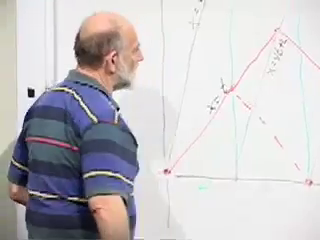
\includegraphics[width=0.72\textwidth]{lecture_01_figure_04.png}
\caption{Der vorwärts laufende Lichtstrahl \(x=t\) schneidet die mittlere Weltlinie des bewegten Gitters.}
\lectureframe{01:02:33}
\end{figure}

Die vollständige Geometrie lässt sich auch zeichnen, ohne dass eine Person an der Tafel im Weg steht:

\begin{figure}[H]
\centering
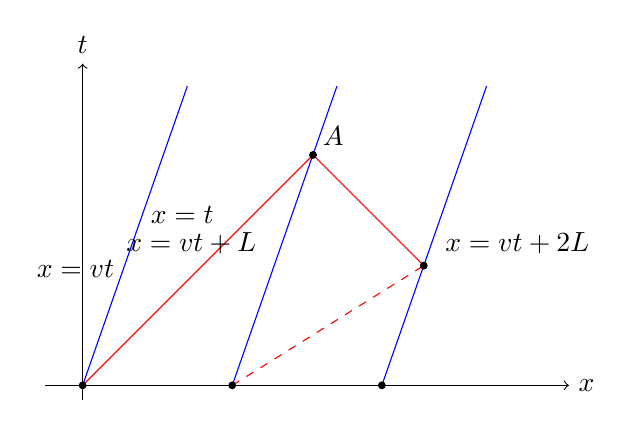
\begin{tikzpicture}[scale=0.95]
\draw[->] (-0.5,0) -- (6.5,0) node[right] {$x$};
\draw[->] (0,-0.2) -- (0,4.3) node[above] {$t$};
\draw[blue] (0,0) -- (1.4,4.0);
\draw[blue] (2.0,0) -- (3.4,4.0);
\draw[blue] (4.0,0) -- (5.4,4.0);
\draw[red] (0,0) -- (3.08,3.08);
\draw[red] (3.08,3.08) -- (4.56,1.60);
\draw[red,dashed] (2.0,0) -- (4.56,1.60);
\fill (0,0) circle (1.5pt);
\fill (2.0,0) circle (1.5pt);
\fill (4.0,0) circle (1.5pt);
\fill (3.08,3.08) circle (1.5pt);
\fill (4.56,1.60) circle (1.5pt);
\node[left] at (0.55,1.55) {$x=vt$};
\node[left] at (2.45,1.9) {$x=vt+L$};
\node[right] at (4.72,1.9) {$x=vt+2L$};
\node[left] at (1.88,2.28) {$x=t$};
\node[above right] at (3.08,3.08) {$A$};
\end{tikzpicture}
\caption{Lichtsignale bestimmen die Gleichzeitigkeitslinie des bewegten Bezugssystems.}
\end{figure}

Senden wir vom Ursprung einen nach rechts laufenden Lichtstrahl aus. Sei \(A\) sein Schnittpunkt mit der mittleren Weltlinie. Die beiden Gleichungen bei \(A\) lauten
\begin{align}
x&=t,\\
x&=vt+L.
\end{align}
Einsetzen ergibt
\begin{equation}
t=vt+L,
\end{equation}
und damit
\begin{equation}
t_A=x_A=\frac{L}{1-v}.
\label{eq:point-a}
\end{equation}

Von \(A\) aus verfolgen wir einen nach links laufenden Lichtstrahl rückwärts bis zur rechtesten bewegten Weltlinie. Seine Gleichung hat die Form
\begin{equation}
x+t=b.
\end{equation}
Da er durch \(A\) verläuft, legt Gleichung~\eqref{eq:point-a} die Konstante fest:
\begin{equation}
b=x_A+t_A=\frac{2L}{1-v}.
\end{equation}
Damit erfüllt der rückwärts laufende Strahl
\begin{equation}
x+t=\frac{2L}{1-v}.
\label{eq:backward-ray}
\end{equation}

Sein Schnittpunkt mit der rechtesten Weltlinie ergibt sich aus
\begin{align}
x+t&=\frac{2L}{1-v},\\
x&=vt+2L.
\end{align}
Eliminieren wir \(x\), so erhalten wir
\begin{align}
(1+v)t
  &=2L\left(\frac{1}{1-v}-1\right)\\
  &=\frac{2Lv}{1-v},
\end{align}
also
\begin{equation}
t=\frac{2Lv}{1-v^2}.
\end{equation}
Einsetzen in \(x=vt+2L\) ergibt
\begin{equation}
x=\frac{2L}{1-v^2}.
\end{equation}
Die Koordinaten selbst sind weniger wichtig als ihr Verhältnis:
\begin{equation}
\frac{t}{x}=v.
\end{equation}
Somit liegt jedes Ereignis, das den bewegten Uhren zufolge gleichzeitig mit dem Ursprung ist, auf
\begin{equation}
t=vx,
\label{eq:simultaneity-c-one}
\end{equation}
wohingegen der bewegte Ursprung der Linie
\begin{equation}
x=vt.
\label{eq:moving-time-axis}
\end{equation}
folgt. Die beiden Achsen sind symmetrisch um den Lichtstrahl bei \(45^\circ\) geneigt.

Alle Punkte auf \(x=vt\) haben dieselbe gestrichene Ortskoordinate \(x'=0\), während ihre gestrichenen Zeiten variieren. Alle Punkte auf \(t=vx\) haben dieselbe gestrichene Zeit \(t'=0\), während ihre gestrichenen Ortskoordinaten variieren. Die eine Linie ist somit die gestrichene Zeitachse, die andere die gestrichene Ortsachse. Die aufwendige Signalkonstruktion war nötig, um die zweite Linie zu bestimmen; aus der Weltlinie des bewegten Ursprungs allein ließ sie sich nicht ableiten.

Um in Gleichung~\eqref{eq:simultaneity-c-one} die gewöhnlichen Einheiten wieder einzusetzen, braucht man
\begin{equation}
t=\frac{v}{c^2}x.
\label{eq:simultaneity-dimensional}
\end{equation}
Der Faktor \(c^2\) erklärt, weshalb das Newtonsche Bild im Alltag so gut funktioniert. Für Geschwindigkeiten, die sehr klein gegenüber \(c\) sind, ist die Neigung der bewegten Gleichzeitigkeitslinie äußerst gering.

\begin{figure}[H]
\centering
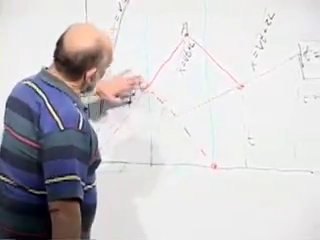
\includegraphics[width=0.72\textwidth]{lecture_01_figure_05.png}
\caption{Bei \(c=1\) sind die gestrichenen Zeit- und Gleichzeitigkeitsachsen symmetrisch zum Lichtstrahl.}
\lectureframe{01:15:40}
\end{figure}

\begin{figure}[H]
\centering
\begin{tikzpicture}[scale=1.0]
\draw[->] (-2.2,0) -- (5.2,0) node[right] {$x$};
\draw[->] (0,-0.2) -- (0,4.9) node[above] {$t$};
\draw[red] (0,0) -- (3.9,3.9);
\draw[red] (0,0) -- (-1.8,1.8);
\draw[blue] (0,0) -- (1.8,4.5);
\draw[blue,dashed] (0,0) -- (4.5,1.8);
\node[right] at (3.9,3.9) {$x=t$};
\node[left] at (-1.8,1.8) {$x=-t$};
\node[above] at (1.8,4.5) {$x'=0$};
\node[right] at (4.5,1.8) {$t'=0$};
\end{tikzpicture}
\caption{Die gestrichenen Achsen und invarianten Lichtstrahlen in Einheiten mit \(c=1\).}
\end{figure}

\section{Herleitung der Lorentz-Transformation}

Die Geometrie legt fest, wo jede gestrichene Koordinate verschwindet. Auf der bewegten Zeitachse \(x=vt\) muss \(x'=0\) gelten. Auf der bewegten Gleichzeitigkeitsachse \(t=vx\) muss \(t'=0\) gelten. Die allgemeinsten linearen Beziehungen mit diesen Nullstellen lassen sich schreiben als
\begin{align}
x'&=\frac{x-vt}{F(v)},\\
t'&=\frac{t-vx}{G(v)}.
\label{eq:fg-ansatz}
\end{align}
Die Faktoren \(F\) und \(G\) erlauben, dass sich die Skalen der gestrichenen Koordinaten von den Galileischen Skalen unterscheiden, obwohl die Achsen bereits festgelegt sind. Die Linearität folgt aus der Homogenität von Raum und Zeit: Eine Verschiebung des Experiments kann das Transformationsgesetz nicht ändern.\editorialnote{Dieses kurze Linearitätsargument macht eine Annahme explizit, die bei der Herleitung an der Tafel implizit verwendet wurde.}

Bis hierhin hat uns die Geometrie vieles, aber noch nicht alles mitgeteilt. Die Zähler legen die Neigung der Achsen fest. Sie bestimmen nicht den Einheitenabstand entlang dieser Achsen. Genau für diese noch fehlende Skalierungsinformation stehen \(F(v)\) und \(G(v)\).

Nun fordern wir die Invarianz der Lichtgeschwindigkeit. Ein nach rechts laufender Strahl, der \(x=t\) erfüllt, muss auch \(x'=t'\) erfüllen. Entlang dieses Strahls gilt
\begin{align}
x'&=\frac{(1-v)t}{F(v)},\\
t'&=\frac{(1-v)t}{G(v)}.
\end{align}
Die Gleichheit für jeden Punkt auf dem Strahl verlangt
\begin{equation}
F(v)=G(v).
\end{equation}
Wir können daher schreiben
\begin{align}
x'&=\frac{x-vt}{F(v)},\\
t'&=\frac{t-vx}{F(v)}.
\label{eq:common-f}
\end{align}

Dieser Schritt bringt die erste wirklich Einsteinische Forderung in die Algebra ein. Dieselbe geometrische Linie ist für beide Beobachter ein Lichtstrahl; daher müssen die beiden gestrichenen Koordinaten entlang dieser Linie gleich stark zunehmen, wenn \(c=1\). Unterschiedliche Faktoren in den beiden Gleichungen würden dazu führen, dass sich die gestrichene Geschwindigkeit von eins unterscheidet.

Eine unbekannte Funktion bleibt noch. Multiplizieren wir Gleichung~\eqref{eq:common-f} mit \(F(v)\):
\begin{align}
F(v)x'&=x-vt,\\
F(v)t'&=t-vx.
\end{align}
Multiplizieren wir die zweite Gleichung mit \(v\) und addieren sie zur ersten, fällt \(t\) heraus. Damit ergibt sich
\begin{equation}
(1-v^2)x=F(v)(x'+vt').
\end{equation}
Entsprechend folgt
\begin{equation}
(1-v^2)t=F(v)(t'+vx').
\end{equation}
Die inverse Transformation lautet somit
\begin{align}
x&=\frac{F(v)}{1-v^2}(x'+vt'),\\
t&=\frac{F(v)}{1-v^2}(t'+vx').
\end{align}

Das Relativitätsprinzip macht die beiden Bezugssysteme wechselseitig gleichberechtigt. Sieht der Bahnhof den Zug mit \(+v\) fahren, so sieht der Zug den Bahnhof mit \(-v\) fahren. Die inversen Gleichungen müssen deshalb dieselbe Form wie die Vorwärtstransformation haben, wobei das Vorzeichen von \(v\) umgekehrt ist. Die Vorfaktoren müssen also erfüllen:
\begin{equation}
\frac{F(v)}{1-v^2}=\frac{1}{F(v)}.
\end{equation}
Daraus folgt
\begin{equation}
F(v)^2=1-v^2,
\end{equation}
und die Stetigkeit mit der Identitätstransformation bei \(v=0\) wählt die positive Wurzel:
\begin{equation}
F(v)=\sqrt{1-v^2}.
\end{equation}

Es wurde nichts an einen bestimmten Lichtimpuls angepasst. Das Ergebnis folgt aus den durch Synchronisation festgelegten Achsen, der gemeinsamen Lichtgeschwindigkeit und der Forderung, dass keines der beiden Inertialsysteme gegenüber dem anderen ausgezeichnet sein darf.

Die Lorentz-Transformation in Einheiten mit \(c=1\) lautet
\begin{align}
x'&=\frac{x-vt}{\sqrt{1-v^2}},\\
t'&=\frac{t-vx}{\sqrt{1-v^2}}.
\label{eq:lorentz-c-one}
\end{align}
Ihre inverse Transformation ist
\begin{align}
x&=\frac{x'+vt'}{\sqrt{1-v^2}},\\
t&=\frac{t'+vx'}{\sqrt{1-v^2}}.
\end{align}

\begin{figure}[H]
\centering
\includegraphics[width=0.76\textwidth]{lecture_01_figure_06.png}
\caption{Die vollständige Lorentz-Transformation für \(c=1\) an der Tafel.}
\lectureframe{01:32:38}
\end{figure}

Die wesentliche Neuerung zeigt sich bereits in der Zeitgleichung. Die Zeit wird nicht einfach unverändert von einem Bezugssystem ins andere übertragen. Eine gestrichene Zeitkoordinate enthält sowohl ungestrichene Zeit als auch den ungestrichenen Ort. Folglich beschreiben \(t=\text{constant}\) und \(t'=\text{constant}\) unterschiedliche Ereignismengen.

Der Mischungsterm ist keine optionale, nachträglich angefügte Korrektur. Ohne ihn bliebe die Linie \(t'=0\) horizontal, die Gleichzeitigkeit entfernter Ereignisse wäre weiterhin universell, und die Transformation könnte die Lichtgeschwindigkeit nicht erhalten.

\section{Lichtgeschwindigkeit wieder einsetzen und das Ergebnis überprüfen}

Für \(c\ne1\) stellt die Dimensionskonsistenz die fehlenden Faktoren wieder her. Das Verhältnis \(v^2/c^2\) ist dimensionslos, während \((v/c^2)x\) die Dimension einer Zeit hat. Somit gilt
\begin{align}
x'&=\frac{x-vt}{\sqrt{1-v^2/c^2}},\\
t'&=\frac{t-(v/c^2)x}{\sqrt{1-v^2/c^2}}.
\label{eq:lorentz-dimensional}
\end{align}
Die inverse Transformation erhält man, indem man das Vorzeichen von \(v\) umkehrt:
\begin{align}
x&=\frac{x'+vt'}{\sqrt{1-v^2/c^2}},\\
t&=\frac{t'+(v/c^2)x'}{\sqrt{1-v^2/c^2}}.
\end{align}
Die Einführung von
\begin{equation}
\gamma=\frac{1}{\sqrt{1-v^2/c^2}}
\end{equation}
würde die vertraute kompakte Form ergeben; die Schreibweise mit dem Nenner macht jedoch die Herleitung besser nachvollziehbar.

Numerisch ist \(c\simeq3\times10^8\,\mathrm{m/s}\), also \(c^2\simeq9\times10^{16}\,\mathrm{m^2/s^2}\). Der große Nenner macht sowohl die Neigung der Gleichzeitigkeitslinie als auch den Faktor \(v^2/c^2\) bei den meisten mechanischen Experimenten unmerklich. Diese geringe Größe erklärt Galileis Erfolg; sie stellt die absolute Zeit nicht wieder her.

\begin{figure}[H]
\centering
\includegraphics[width=0.76\textwidth]{lecture_01_figure_07.png}
\caption{Die Lorentz-Transformation mit wieder eingesetzten Faktoren von \(c\).}
\lectureframe{01:35:58}
\end{figure}

Zwei Überprüfungen liegen unmittelbar nahe. Betrachten wir zunächst \(v\ll c\). Dann ist \(v^2/c^2\) vernachlässigbar, und bei gewöhnlichen Entfernungen ist auch der Term der Relativität der Gleichzeitigkeit \(vx/c^2\) vernachlässigbar. Gleichung~\eqref{eq:lorentz-dimensional} vereinfacht sich zu
\begin{equation}
t'\approx t,\qquad x'\approx x-vt.
\end{equation}
Die Galilei-Relativität ergibt sich als Näherung für niedrige Geschwindigkeiten.

Prüfen wir zweitens einen Lichtstrahl. Nachdem \(c\) wieder eingesetzt wurde, erfüllt ein nach rechts laufender Strahl \(x=ct\), nicht \(x=t\). Einsetzen ergibt
\begin{align}
x'&=\frac{(c-v)t}{\sqrt{1-v^2/c^2}},\\
t'&=\frac{(1-v/c)t}{\sqrt{1-v^2/c^2}}.
\end{align}
Da \(c-v=c(1-v/c)\) gilt,
\begin{equation}
x'=ct'.
\end{equation}
misst der gestrichene Beobachter dieselbe Geschwindigkeit \(c\). Für einen nach links laufenden Strahl ergibt das Einsetzen von \(x=-ct\) entsprechend
\begin{equation}
x'=-ct'.
\end{equation}
Die Transformation behandelt Licht, das sich in beide Richtungen ausbreitet, korrekt.

Die Unterscheidung zwischen \(x=t\) und \(x=ct\) ist eine lehrreiche Dimensionsprüfung. Der erstere Ausdruck ist nur in Einheiten korrekt, in denen \(c=1\) gilt. Würde man in der Transformation die gewöhnlichen Einheiten wieder einsetzen, die Strahlgleichung aber in natürlichen Einheiten belassen, vermischte man zwei Konventionen und erhielte ein falsches Ergebnis. Die Dimensionskonsistenz deckt den Fehler sofort auf.

\section{Das Mittelpunktkriterium}

\begin{classroomqa}
\audiencequestion{Angenommen, ein Beobachter empfängt zwei Lichtblitze gleichzeitig, befindet sich aber nicht auf halbem Weg zwischen ihren Quellen. Kann dieser Beobachter daraus schließen, dass die Blitze gleichzeitig ausgesendet wurden?
\lecturetimestamp{01:42:55}}
\lecturerresponse{Nein. Gleiche Ankunftszeiten bedeuten nur für den Beobachter gleiche Aussendezeiten, der sich im betreffenden Bezugssystem räumlich genau zwischen den beiden Quellen befindet. Ein Empfänger, der einer Quelle näher ist, kann beide Blitze gleichzeitig empfangen, obwohl der weiter entfernte Blitz früher ausgesendet wurde. In der bewegten Konstruktion ist die Weltlinie des Mittelpunkts \(x=vt+L\) daher wesentlich. Dem Vorwärtsstrahl \(x=t\) folgt man, bis er diesen Mittelpunkt erreicht, und anschließend verfolgt man einen rückwärts laufenden Lichtstrahl bis \(x=vt+2L\). Dieses zweite Endereignis ist nach dem bewegten Bezugssystem gleichzeitig mit dem Ursprung, nicht etwa ein beliebiges Ereignis an einem anderen Ort mit gleicher Ankunftszeit.}
\end{classroomqa}

Wir haben die vollständige Koordinatentransformation erreicht, aber noch nicht ihre bekanntesten Folgerungen. Als Nächstes folgen die Längenkontraktion, die Zeitdilatation und die Eigenzeit, danach relativistischer Impuls und relativistische Energie. Die Grundlage ist bereits gelegt: Jedes Inertialsystem kann dieselben Gesetze verwenden und dieselbe Lichtgeschwindigkeit messen, weil sich Raum und Zeit miteinander vermischen und weil die Gleichzeitigkeit entfernter Ereignisse zu einem Bezugssystem gehört und nicht absolut zur Welt.